\chapter{Arbeid}
\begin{blockquotebox}
    Het inzetten van fysiologische functies en uitingen van het menselijk leven als middel noemen we arbeid. De mens werkt door zijn krachten en vaardigheden in te zetten als middel om ongemak te verminderen en door doelgericht gebruik te maken van zijn levensenergie, voor de spontane en zorgeloze  ontlasting van zijn capaciteiten en zenuwstelsel. Arbeid is een middel, geen doel op zich. Elk individu heeft slechts een beperkte hoeveelheid energie om te besteden, en elke eenheid arbeid kan slechts een beperkt effect teweegbrengen. Anders zou menselijke arbeid in overvloed beschikbaar zijn; zij zou niet schaars zijn, noch worden beschouwd als een productiemiddel om ongemak te verlichten en als zodanig op worden behandeld.\footnotemark \par\raggedleft--- Ludwig von Mises\index{Ludwig von Mises}
\end{blockquotebox}
\footautocite{37}

\section{Arbeid en vrije tijd}

\lettrine{M}enselijke tijd is het ultieme en schaarste\index{schaarste} middel. Eenmaal gespendeerd
is het onherstelbaar, en de hoeveelheid kan niet eindeloos worden
vergroot. De schaarste\index{schaarste} en onvoorspelbaarheid van tijd creëren bij mensen
een positieve tijdsvoorkeur\index{tijdsvoorkeur}: een voorkeur voor een huidig goed boven een
identiek goed in de toekomst. Deze voorkeur geldt voor tijd zelf. Mensen
waarderen hun huidige tijd meer dan identieke tijd in de toekomst.
Tijdsvoorkeur varieert in de loop van een leven en van persoon tot
persoon, maar is toch altijd aanwezig en altijd positief.

We kunnen onze tijd op twee manieren besteden. De eerste bestaat uit het
doen van dingen die we verlangen, leuk vinden en willen doen omwille van
zichzelf. We zeggen dat ze nut leveren op zich, omdat ze subjectief
waardevol zijn voor de individuen die ze ondernemen. Ze zijn in zekere
zin hun eigen beloning. Economen noemen deze tijdsbesteding
\textbf{vrije tijd}, wat rust, tijd met geliefden, vermaak en recreatie
omvat. Vrije tijd is wat je zou doen als je niet hoefde te werken. De
tweede manier om tijd te besteden is door dingen te doen omwille van
zijn resultaten en uitkomsten. Dit is tijd die een mens besteedt aan
activiteiten die hij op zichzelf niet waardevol vindt, maar die wel
waardevolle resultaten opleveren. Economen verwijzen naar dit gebruik
van tijd als \textbf{arbeid}, door Mises gedefinieerd als ``het gebruik
van de fysiologische functies en uitingen van het menselijk leven als
productiemiddel.''\autocite{38}

Het onderscheid tussen vrije tijd en arbeid is het onderscheid tussen
wat je \emph{wilt} doen en wat je \emph{moet} doen. Of anders gezegd,
het is het verschil tussen wat je doet omwille van zichzelf en wat je
doet omwille van de verwachte toekomstige resultaten. Als iemand een
activiteit onderneemt, enkel en alleen omdat hij of zij er plezier in
heeft, ongeacht de uitkomst, dan zou het geen arbeid zijn, maar vrije
tijd. Per definitie heeft arbeid op zichzelf een negatief nut of
ongemak. Werken vermindert de menselijke tevredenheid, maar toch gaan we
ermee door omdat we verwachten dat dit resultaten zal opleveren die ons
in de toekomst grotere voldoening geven. Het directe nut van vrije tijd
wordt opgeofferd ten gunste van het verwachte toekomstige nut dat
voortkomt uit de resultaten van de arbeid. \textbf{De
opportuniteitskosten van arbeid zijn de vrije tijd die we opgeven}.

Als ze erg jong zijn, hebben mensen een oneindig hoge tijdsvoorkeur\index{tijdsvoorkeur},
omdat ze niet in staat zijn om arbeid of iets anders dan hun
onmiddellijke basisverlangens te begrijpen. Naarmate mensen opgroeien en
cognitief volwassener worden, beseffen ze dat niet enkel het verhogen
van de waarde van hun huidige tijd van belang is. Zodra kinderen in
staat zijn om over de toekomst na te denken en die te waarderen,
beginnen ze onmiddellijke voldoening uit te stellen in ruil\index{ruil} voor
toekomstige beloningen. Naarmate we ouder worden, start onze waardering
voor de toekomst het proces waarin we onze tijdsvoorkeur\index{tijdsvoorkeur} verlagen. Met
het vermogen om over de toekomst na te denken, komt het vermogen om
erover te redeneren, ervoor te plannen en ervoor te werken. Leren om
zindelijk te worden, of welke activiteit in afwachting van ouderlijke
beloning dan ook, kan de eerste activiteit zijn die een kind leert om
huidige arbeid te ruilen voor toekomstige beloning.

Bij het bereiken van volwassenheid overstijgt de mens de bekrompen zorg
voor directe voldoening en begint hij te economiseren voor de toekomst.
Dit neemt twee vormen aan. Een eerste vorm is het bezuinigen (of
economiseren) om de tijd die hij leeft te verlengen. De tweede vorm
omvat het economiseren om voor zichzelf te kunnen zorgen in toekomstige
perioden in zijn leven. De menselijke strijd om te overleven en te
gedijen is de strijd om de hoeveelheid en waarde van de tijd die we op
aarde doorbrengen te vergroten. Deze strijd is onlosmakelijk verbonden
met de noodzaak om in het heden te werken. Overleven en op de lange
termijn floreren vereist arbeid, net als het opofferen van direct plezier, en
stimuleert het verlagen van onze tijdsvoorkeur\index{tijdsvoorkeur}. Wanneer we de opbrengst
van arbeid meer waarderen dan het ongemak van het opofferen van vrije
tijd, dan zullen we werken.

Het verstand drijft de mens tot het besef dat hij in het heden arbeid
kan verrichten om zichzelf in de toekomst van nut te voorzien, zijn
toekomstige subjectieve welzijn te verbeteren en in leven te blijven.
Ongeacht hoe gunstig of ongunstig zijn omstandigheden zijn, zal de mens
altijd manieren bedenken om zijn situatie te verbeteren. Of het nu in
een tropisch paradijs is, in een woestijn, op een boerderij of in een
moderne industriële samenleving, het verstand zal altijd een manier
vinden om de fysiologische functies en tijd van de mens te sturen in de
richting van het verbeteren van zijn toestand. Er zal nú altijd nut zijn
om op te offeren op het altaar van toekomstig nut, en het menselijke
verstand zal de mens daar altijd toe brengen.

De schipbreukeling die gestrand is op een idyllisch, tropisch
eilandparadijs, lijkt voor de moderne mens misschien het ideale leven te
leiden, maar zo'n leven zal toch onvermijdelijk arbeid
met zich meebrengen. Een mens kan op het strand een tijdje gelukkig
zijn, maar naarmate de tijd verstrijkt, neemt zijn tevredenheid af en
ontstaan er andere behoeften. Tijd op het strand, zoals vrije tijd in
het algemeen en zoals alle goederen met een positief nut, vertoont
afnemende marginale opbrengsten. Het strandplezier neemt af naarmate men
er langer doorbrengt. Andere verlangens worden alleen maar intenser
omdat ze langer onvervuld blijven. De schipbreukeling krijgt al snel
honger en zijn verstand zal hem tot de conclusie leiden dat hij zijn
honger kan stillen door te werken om voedsel te verzamelen. Zijn
verstand leidt hem ertoe manieren te bedenken om wilde dieren om te
zetten in voeding. Hij probeert een vis te vangen met zijn blote handen,
of hij jaagt op konijnen en herten. Er is geen garantie dat zijn harde
werk een waardevolle opbrengst zal opleveren. Maar naarmate de tijd
verstrijkt wordt de honger dringender en de jacht urgenter, en
vermindert de waarde van de vrije tijd die genoten zou kunnen worden
zonder arbeid. Dit geeft een prikkel voor meer, beter en slimmer werk.

De motivatie voor werk is uiteindelijk dat het niet doen, of het niet
succesvol uitvoeren ervan, vroeg of laat tot de dood zal leiden. Buiten
de Hof van Eden heeft de mens altijd moeten werken om te overleven en te
gedijen. Op elk moment staat elk individu voor de keuze tussen arbeid en
vrije tijd, evenals de keuze welk soort arbeid uit te voeren om zijn
productiviteit te verhogen. Arbeid is ons eerste conceptuele middel om
de hoeveelheid en waarde van onze tijd te verhogen. Toch is arbeid niet
iets unieks voor mensen. Dieren hebben instinctief het vermogen om zich
bezig te houden met activiteiten waarvan de beloningen niet onmiddellijk
zijn. Ze ruilen huidig nut in voor toekomstig nut. Vogels bouwen nesten,
bevers bouwen dammen en roofdieren besteden veel tijd aan het
achtervolgen van hun prooi. In tegenstelling tot dierlijke instincten,
kan het menselijk verstand vele andere methoden bedenken om economisch\index{economisch}
te handelen en de productiviteit van onze arbeid te verhogen. In de
volgende hoofdstukken gaan we deze methoden in meer detail bespreken.

De belangrijkste manier waarop mensen hun omgeving beïnvloeden is via
het productieproces\index{productieproces}. De volgende paragraaf definieert de belangrijkste
terminologie van productie\index{productie}, die de basis zal vormen voor de rest van het
boek.

\section{Productie}

\textbf{Productie} wordt door Mises gedefinieerd als de \enquote{verandering van
wat voorhanden is volgens de ontwerpen van het verstand.} Volgens Mises
\enquote{zijn deze ontwerpen -- de recepten, formules, en ideologieën -- het
belangrijkste; ze transformeren de oorspronkelijke factoren -- zowel
menselijk als niet-menselijk -- tot middelen. Mensen produceren dankzij
hun verstand; ze kiezen doelen en gebruiken middelen om deze te
bereiken. De populaire uitspraak dat economie gaat over materiële
omstandigheden van het menselijk leven is volledig misplaatst. Menselijk
handelen is een manifestatie van de geest.}\autocite{39}

\textbf{Arbeid}~is \enquote{het gebruik van de fysiologische functies en
uitingen van het menselijk leven als productiemiddel.}\autocite{40} Mensen werken alleen wanneer ze de verwachte opbrengst van hun arbeid
hoger waarderen dan de misgelopen voldoening die beperking van vrije
tijd veroorzaakt. Werken brengt ongemak met zich mee.

\textbf{Consumptiegoederen, eindproducten of goederen van de eerste
orde} bevredigen de menselijke behoeften rechtstreeks, onafhankelijk van
andere goederen. Dit is het einddoel van het productieproces\index{productieproces} en de reden
waarom het proces wordt ondernomen.

\textbf{Productiegoederen, intermediaire goederen, productiefactoren, of
goederen van hogere orde} zijn goederen die indirect aan de menselijke
behoeften voldoen, als ze worden gebruikt om consumptiegoederen\index{consumptiegoed} te
produceren. Menselijke arbeid kan worden beschouwd als een
productiegoed. Maar deze term wordt doorgaans gebruikt om te refereren
aan \textbf{kapitaal\index{kapitaal}}. Een kapitaalgoed\index{kapitaalgoederen} is elk goed dat wordt verkregen
om andere goederen mee te produceren, niet om op zichzelf zelf te
gebruiken. Het bestaan van een kapitaalgoed\index{kapitaalgoederen} vereist het opofferen van
consumptiegoederen\index{consumptiegoed}.

\textbf{Productiviteit} is de hoeveelheid productie\index{productie} die door één eenheid
input in een bepaalde tijdsperiode wordt geproduceerd.

\textbf{Ruil of handel}: Het opzettelijk vervangen van een minder
bevredigende situatie voor een meer bevredigende. Productie kan worden
begrepen als een ruil\index{ruil} van vrije tijd en kapitaalinvesteringen voor de
opbrengsten van arbeidsproductie.

\textbf{Prijs}: Dat wat wordt opgegeven bij ruil\index{ruil} of handel.

\textbf{Kosten}: De waarde van de prijs\index{prijs}; de waarde van de tevredenheid
die we moeten opgeven om het gewenste doel te bereiken.

\textbf{Winst, opbrengst, of netto rendement}: Het verschil tussen de
waarde van de betaalde prijs\index{prijs} (de gemaakte kosten) en die van het
behaalde doel. Winst in deze primaire betekenis is puur subjectief; het
is een toename van het geluk van de handelende mens, een psychisch
fenomeen dat noch gemeten noch gewogen kan worden.


\section{Arbeidsproductiviteit}

Een mens kan werken om producten voor zichzelf te produceren, of hij kan
werken om producten voor anderen te maken, waarbij hij compensatie
ontvangt in ruil\index{ruil} voor zijn tijd. Loonarbeid verschilt van het verrichten
van een dienst voor iemand als gunst of geschenk, omdat er bij
loonarbeid sprake is van compensatie. Loonarbeid verschilt van
slavenarbeid doordat het vrijwillig is; de arbeider kan stoppen met
werken en de werkgever kan alleen proberen hem te behouden door hem te overhalen om vrijwillig terug te keren met stimulansen zoals
betere betaling, betere werkomstandigheden of vergelijkbare
niet-dwingende middelen. Arbeid is per definitie een wederzijdse
overeenkomst tussen de werknemer en de werkgever.

De beslissing van een werkgever om een werknemer aan te nemen, kan worden gezien als een markttransactie zoals elke andere. Het onderscheid met de verhandeling van een consumptiegoed ligt in het feit dat werkgevers arbeid niet beoordelen op basis van hun persoonlijke subjectieve voorkeuren, aangezien arbeid voor hen geen consumptiegoed\index{consumptiegoed} vertegenwoordigt. Omdat arbeid een productiemiddel is, bepaalt de werkgever de waarde van arbeid op grond van de hoeveelheid output die het kan genereren, vermenigvuldigd met de subjectieve waarde die de markt hecht aan het voortgebrachte product.

Werkgever en werknemer kunnen alleen vrijwillig instemmen met een
regeling om arbeid tegen betaling te ruilen als ze beiden tevreden zijn
met de voorwaarden van de ruil\index{ruil}. Voor de arbeider betekent dit dat zijn
compensatie hoger is dan zijn waardering van het alternatieve gebruik
van zijn tijd, wat vrije tijd of een andere, betere baan kan zijn. Voor
de werkgever moet de waarde van de arbeid van de werknemer ook groter
zijn dan het betaalde loon, anders zou de werkgever het niet betalen.
Onderaan de streep, besluit een werkgever alleen om een extra arbeider
in te huren, als die een marginale toename in opbrengst biedt die hoger
is dan het betaalde loon. Elke extra werknemer moet bijdragen tot een
toename van de marginale productie\index{productie}. De marginale toename in de
geproduceerde hoeveelheid wordt het marginale product van de werknemer
genoemd. Wanneer dat getal wordt vermenigvuldigd met de prijs\index{prijs} van het
product, verkrijgen we de \textbf{marginale opbrengst}, een maat voor de
marginale inkomsten die de werknemer voor de werkgever oplevert. Als het
loon hoger is dan de waardering van de werknemer voor vrije tijd of het
beste alternatief voor zijn tijd, en lager is dan de marginale opbrengst
voor de werkgever, dan kunnen beiden overeenkomen om samen te werken en
een wederzijds voordeel te behalen. In alle andere gevallen zal geen
ruil\index{ruil} van arbeid voor compensatie tussen de twee partijen plaatsvinden.

Arbeid heeft een unieke plaats in onze wereld, vanwege wat Mises het
\enquote{niet-specifieke karakter} noemt.\autocite{41} In tegenstelling tot gespecialiseerde
kapitaalgoederen\index{kapitaalgoederen} kan menselijke tijd op veel soorten
productieprocessen worden gericht. Kapitaal dat in een specifieke
bedrijfstak niet langer productief is, zal waarschijnlijk
overbodig raken, maar menselijke tijd kan altijd opnieuw worden
hergebruikt voor productieve doeleinden. Door de ultieme schaarste\index{schaarste} van
menselijke tijd is er wereldwijd altijd meer vraag naar meer menselijke
hersenen en handen om te werken. Werkgevers zijn altijd bereid
om de volgende werknemer in dienst te nemen tegen een loon dat lager is
dan hun marginale productiviteit.

Productiviteit wordt gedefinieerd als de hoeveelheid output die geproduceerd wordt door een enkele eenheid van input binnen een specifieke tijdspanne. Zoals besproken in het voorgaande hoofdstuk, is de waarde van menselijke tijd door de geschiedenis heen aanzienlijk toegenomen. Naarmate de tijd vordert, nemen de reële lonen toe omdat de productiviteit van werknemers blijft verbeteren. Dit motiveert werkgevers om hogere lonen te bieden om de benodigde arbeidskrachten aan te trekken en te behouden, en om te voorkomen dat zij overstappen naar concurrenten.

In de afgelopen 200 jaar is de waarde van
menselijke tijd met de Industriële Revolutie continu gestegen. Mensen hebben meer kapitaal\index{kapitaal}
geaccumuleerd, productievere technologieën uitgevonden, krachtigere
energiebronnen gebruikt en de arbeidsdeling\index{arbeidsdeling} uitgebreid naar grotere
markten\index{markten} en meer deelnemers. Alle uitvindingen, gereedschappen en
technologieën die de menselijke productiviteit verhogen, hebben geleid
tot een langer menselijk leven en een toename van de waarde van onze
tijd. We moeten nu immers aanzienlijk meer betaald worden om afstand te
doen van onze vrije tijd. Het uiteindelijke doel van economisch\index{economisch} handelen is om mensen meer en een betere tijd op aarde te geven.

\section{Werkloosheid}

In de twintigste eeuw raakten het concept van werkloosheid en het
concept van arbeid nauw met elkaar verweven. Veel denkstromingen hebben
gesteld dat werkloosheid een onvermijdelijk en onontkoombaar onderdeel
is van de economische marktwerking. Er zijn verschillende redenen
aangevoerd om uit te leggen waarom een vrije arbeidsmarkt onvermijdelijk
zal falen op een manier die velen die wel bereid zijn om te werken tegen
de gangbare lonen, werkloos laat.

Maar werkloosheid is net zo een normaal onderdeel van de arbeidsmarkt
als het verbranden van oogsten een onderdeel is van de voedselmarkt.
Zoals in Hoofdstuk IV van dit boek zal worden besproken, zijn inflatoire
kredietexpansie en wetten voor minimumloon de hoofdoorzaak van
werkloosheid. Inflatie leidt tot stijging van de prijzen, waardoor
werknemers om hogere lonen vragen om hun stijgende kosten van
levensonderhoud te dekken. Maar omdat een toename in een monetair middel
geen toename in economische middelen met zich meebrengt, hebben
werkgevers vaak geen mogelijkheid om hun werknemers hogere lonen te
betalen en tegelijkertijd in bedrijf\index{bedrijf} te blijven. Ze moeten dan of
werknemers ontslaan, of het bedrijf\index{bedrijf} sluiten. Inflatie verlaagt welvaart
en vermogens van zowel de werknemer als de werkgever, en verhoogt de
prijs\index{prijs} van de producten die ze op de markt willen kopen. Bovendien is
kredietinflatie ook de oorzaak van de conjunctuurcyclus\index{conjunctuurcyclus}. Een inflatoire
boom leidt tot de financiering van onhoudbare investeringen, en hun
onvermijdelijke ineenstorting leidt tot het faillissement\index{faillissement} van hele
economische sectoren, met grote aantallen werknemers die worden
ontslagen en achterblijven met vaardigheden waar weinig vraag naar is.

Inflatie\index{inflatie} leidt tot werkloosheid door de combinatie van stijgende prijzen en recessies. Overheden en door hen aangestelde economen wijzen vaak de markteconomie zelf of ``hebzuchtige'' kapitalisten aan als zondebok, of ze komen met andere excuses. In plaats van inflatie aan te pakken in de kern van het probleem, adviseren moderne economen vaak contraproductieve maatregelen, zoals wetgeving voor een minimumloon. Deze maatregelen moeten niet gezien worden als een verplichting voor werkgevers om hun werknemers meer te betalen, maar eerder als een restrictie die werknemers belet om zelf de prijs van hun arbeid te bepalen. Wetten omtrent minimumloon belemmeren de aanpassing van de markt aan inflatie, wat leidt tot aanhoudende golven van werkloosheid die parallel lopen met de conjunctuurcyclus\index{conjunctuurcyclus}.

Het is opmerkelijk dat het begrip werkloosheid vóór de twintigste eeuw
niet echt bestond als economische term. In een vrije markt kiezen mensen
ervoor om wel of niet te werken voor het aangeboden loon, dus niemand
kan tegen zijn wil werkloos zijn. Met de invoering van monetaire
inflatie\index{inflatie} en minimumloonwetten werd een permanent werkloos deel van de
bevolking een vast onderdeel van de moderne economie. De schuld voor de
werkloosheid werd toegeschreven aan de markt, kenmerkend voor de
dominante, pseudowetenschappelijke economische stroming in de moderne
academische wereld. Dit wordt gefinancierd door mensen die belang hebben
bij het in stand houden van inflatie\index{inflatie}.

Zwitserland, als het laatste land ter wereld dat de goudstandaard\index{goudstandaard} verliet, illustreert deze dynamiek treffend. Gedurende de gehele twintigste eeuw, terwijl de rest van de wereld kampte met ernstige werkloosheidscrisissen onder een fiatgeldsysteem\index{fiatgeld}, kende Zwitserland nauwelijks werkloosheid tot het midden van de jaren 70, toen het de goudstandaard opgaf.\autocite{42} Na de overstap op de dollarstandaard en het toestaan van inflatie\index{inflatie}, werd Zwitserland geconfronteerd met toenemende werkloosheid, die hetzelfde cyclische patroon volgde dat in elk land zichtbaar is dat gebruikmaakt van fiatgeld.

\begin{figure}[!htb]
\centering
    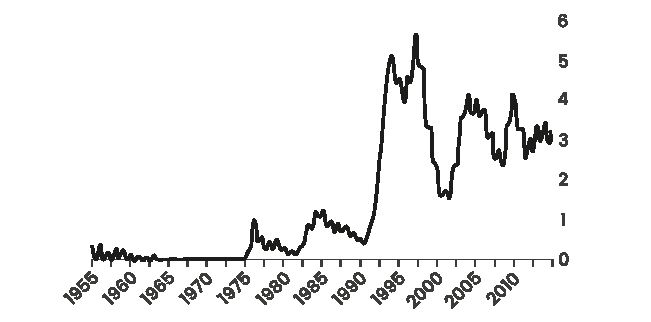
\includegraphics[width=\textwidth]{figures/fig7.pdf}
\caption[Werkloosheidspercentage in Zwitserland]{Werkloosheidspercentage in Zwitserland}
\label{fig7}
\end{figure}

In een vrije markt met gezond geld\index{gezond geld} neemt spaargeld gedurende de tijd in
marktwaarde toe, en hebben individuen de vrijheid om wel of niet te
werken. Ze kunnen elk gewenst loon vragen. Werkgevers hebben ook de
vrijheid om elk gewenst salaris te betalen. In zo'n
wereld waarin spaartegoeden\index{spaartegoeden} in waarde stijgen, is het volkomen rationeel
dat velen ervoor kiezen om geen werk te zoeken. Een werknemer die geen
werk kan vinden tegen een geldend loon, kan simpelweg niemand vinden die
de marginale opbrengst van zijn arbeid hoger waardeert dan de werknemer
zijn persoonlijke waardering van vrije tijd. Het moderne fenomeen van
massale, onvrijwillige werkloosheid is alleen mogelijk wanneer wetten,
regels of beperkingen bestaan die het illegaal en strafbaar maken om
arbeid te verrichten tegen specifieke loonniveaus.

In de context van vrije handel kan er onder mensen die bereid zijn om te
werken geen sprake zijn van werkloosheid, aangezien dat zou betekenen
dat ze recht hebben op een loon dat niemand bereid is hen te betalen. De
werknemer zou altijd werk kunnen vinden door zijn productiviteit te
verhogen of zijn gevraagde loon te verlagen. Gedwongen werkloosheid is
onmogelijk in een vrijemarkteconomie; het is de keuze van de werknemer
om een loon te vragen dat niemand bereid is te betalen, en daardoor is
het hun keuze om werkloos te blijven.

\section{Komt er ooit een einde aan werk?}

Arbeid is als productiemiddel uiterst waardevol, juist omdat het met
vrije tijd concurreert om het meest schaarse productiemiddel, de
menselijke tijd. Naarmate het inkomen en nut dat je door werk krijgt toeneemt, neemt de welvaart van werknemers toe. Dit stelt hen in staat
zich meer vrije tijd te veroorloven, maar het vergroot ook de
vermindering van het nut van hun arbeid en ontmoedigt hen om te werken.
Arbeid zou het enige economische goed of activiteit kunnen zijn waarvan
de geleverde hoeveelheid kan afnemen naarmate de prijs\index{prijs} stijgt. Dit komt
doordat een stijging van de arbeidsprijs leidt tot een toename van de
rijkdom van de werknemer, waardoor hij meer vrije tijd kan kopen en
minder arbeid hoeft te verkopen. De schaarste\index{schaarste} aan tijd betekent dat het
aanbieden van arbeid opportuniteitskosten met zich meebrengt die
toenemen naarmate een persoon meer verdient met werken. Deze dynamiek
heeft velen doen speculeren dat economische vooruitgang op een dag zou
kunnen betekenen dat mensen niet meer hoeven te werken.

Zullen we ooit een punt bereiken waarop we niet meer hoeven te werken?
Dit is een veel voorkomende fantasie onder politici en economen die niet
vertrouwd zijn met de economische manier van denken, zoals John Maynard
Keynes en zijn vele volgelingen. In de jaren `30 speculeerde Keynes dat
de productiviteit zo sterk zou blijven stijgen dat mensen tegen 2030
slechts 15 uur per week zouden moeten werken om te produceren wat ze
nodig hebben. Keynes fantaseerde dat technologische vooruitgang zou
leiden tot technologische werkloosheid, die hij definieerde als
\enquote{werkloosheid door onze ontdekking van middelen om sneller op het
gebruik van arbeid te besparen dan het tempo waarin we nieuwe
toepassingen voor arbeid kunnen vinden.}\autocite{43}

\enquote{Dit alles betekent op de lange termijn dat de mensheid haar economisch\index{economisch}
probleem oplost}, concludeerde Keynes. Hij zag het economisch\index{economisch} vraagstuk
als een wiskundig probleem dat maar éénmaal opgelost hoeft te worden om
definitief opgelost te zijn. Hij ging ervan uit dat het vooral draaide
om het veiligstellen van een bepaalde verzameling goederen en diensten
die nodig zijn voor een gelukkig leven. Wanneer daar eenmaal voor was
gezorgd, zou het economisch\index{economisch} probleem voor eens en altijd zijn opgelost,
waardoor niemand ooit meer economisch\index{economisch} zou hoeven te handelen. In
werkelijkheid is het economisch\index{economisch} vraagstuk een permanent onderdeel van
het menselijk bestaan. We worden voortdurend geconfronteerd met keuzes
tussen schaarse dingen, omdat die schaarste\index{schaarste} voortkomt uit onze beperkte
en extreem kostbare tijd. Zolang mensen leven en moeten beslissen hoe ze
hun tijd willen besteden, zal het economische vraagstuk blijven bestaan
en zullen mensen het proberen op te lossen door te werken. Er kan geen
definitieve oplossing zijn voor het economisch\index{economisch} vraagstuk, alleen de
vervanging van slechte keuzes door betere keuzes.

\enquote{Ik concludeer dat, ervan uitgaande dat er geen belangrijke oorlogen en
geen belangrijke bevolkingsgroei zullen zijn, het economisch\index{economisch} probleem
binnen honderd jaar opgelost kan zijn, of op z'n minst
een oplossing in zicht is... Dus voor de eerste keer sinds zijn
schepping zal de mens worden geconfronteerd met zijn echte en permanente
probleem -- hoe hij zijn vrij zijn van dringende economische zorgen moet
gebruiken, hoe hij de vrije tijd, die wetenschap en samengestelde rente\index{rente}
hebben voortgebracht, moet besteden om wijs, aangenaam en goed te
leven.}\autocite{45}

Keynes lijkt zich niet bewust te zijn van het feit dat wat hij voorstelt
als een vervanging voor het economisch\index{economisch} probleem, gewoon het economisch\index{economisch}
probleem zelf is, maar dan toegepast op keuzes die iets anders zijn dan
die hij gewend was te zien in de zeer weinige economische boeken die hij
had gelezen. Het eeuwige en universele economische probleem van de mens
is hoe we onze tijd besteden, omdat tijd schaars is. De simplistische
opvatting van Keynes over de economie maakt het hem onmogelijk te
onderkennen dat het gebruik van tijd een economische keuze is.

Ongeacht hoeveel materiële dingen we hebben, we zullen altijd een keuze
moeten maken in de marge van directe en toekomstige voldoening. We
kunnen altijd huidige voldoening opgeven voor meer toekomstige
voldoening. Er zal nooit volledige voldoening zijn, omdat het menselijk
verstand altijd een betere mogelijkheid zal voorzien en ernaar zal
streven. Het zou voor iemand heel goedkoop zijn om vandaag te leven
volgens de levensstandaard van Keynes' tijd. Toch
kunnen zelfs de armste mensen vandaag de dag veel dingen gebruiken en
bezitten die Keynes nooit heeft kunnen bezitten. En ze blijven verlangen
naar een beter leven, net als de rijkste mensen. Zolang mensen
economisch\index{economisch} handelen, gebruiken ze hun verstand om nieuwe goederen,
diensten en objecten te produceren die anderen wensen.

Keynes baseert zijn fantasierijke visie van de toekomst op een volledig
ongegronde bewering dat er twee soorten behoeften zijn: absolute en
relatieve behoeften. Absolute behoeften, zo stelde Keynes, zijn
behoeften die we voelen \enquote{ongeacht de situatie van onze medemensen}.
Daarentegen worden relatieve behoeften alleen gevoeld \enquote{als hun
vervulling ons boven onze medemensen uit tilt, ons een gevoel van
superioriteit geeft}.\autocite{46} Keynes stelt dat de vraag naar het voldoen 
van het laatste wellicht onverzadigbaar zou kunnen zijn, maar dat aan de vraag 
naar de vervulling van de eerste klasse van behoeften volledig voldaan zou 
kunnen worden. Keynes dacht dat het economisch\index{economisch} probleem altijd het primaire en
dringendste probleem van het menselijk ras en het hele biologische rijk
is geweest. Het oplossen ervan zou een buitengewoon belangrijke
verandering in de aard van het menselijk leven betekenen. Hij begreep
echter niet dat het economisch\index{economisch} probleem altijd bestaat zolang menselijke
tijd schaars is en mensen keuzes moeten maken. Zelfs als mensen zich in
een denkbeeldige wereld bevonden waarin alles wat ze zich wensen
onmiddellijk wordt gerealiseerd, dan nog zou het economisch\index{economisch} probleem
niet zijn opgelost. De sterfelijkheid van de mensen dwingt hen nog
steeds om economisch\index{economisch} met hun schaarse tijd om te gaan. Het economisch\index{economisch}
probleem wordt elke seconde opgelost wanneer een mens nadenkt over zijn
tijd en een keuze maakt. Maar dan dient zich in de volgende seconde een
nieuw economisch\index{economisch} probleem aan dat dezelfde mens dwingt om opnieuw een
keuze te maken. De enige definitieve oplossing voor het economisch\index{economisch}
probleem is de dood, het moment waarop er geen verdere keuzes meer zijn
over de verdeling van de tijd.

Het is dus onzinnig om je zoals Keynes voor te stellen dat werk
ooit zou kunnen stoppen, of dat de behoefte aan werk ooit zou kunnen
verdwijnen, of dat overvloed een punt zou bereiken waarop arbeid niet
meer nodig is. We handelen voortdurend economisch\index{economisch} en we moeten altijd
keuzes maken tussen alternatieven. Naarmate onze levensstandaard
verbetert, verbeteren onze keuzes, maar het maken van keuzes moet
blijven bestaan, in ieder geval zolang mensen sterfelijk zijn.

\section{Is werk uitbuiting?}

Worden arbeiders uitgebuit door het kapitalisme\index{kapitalisme}? Er zijn miljoenen
pagina's geschreven over het onderwerp van uitbuiting
van arbeiders, voornamelijk gebaseerd op het onsamenhangende gewauwel
van Karl Marx. Marx was een semi-geletterde Duitse zwerver die nooit een
baan had die hem kon onderhouden. Marx leefde van de steun van rijke weldoeners 
terwijl hij orakelde over het herontwerpen van de wereld tot een dystopie, 
geleid door mensen die niet in staat zijn zichzelf te onderhouden door hun eigen arbeid.

Marxistische economische analyse is gebaseerd op de arbeidswaardeleer,
besproken in Hoofdstuk 2. Aangezien alle economische goederen arbeid
vereisen om ze te veranderen in bruikbare economische goederen,
concludeert de marxist ten onrechte dat arbeid economische goederen
waarde geeft en dat de hoeveelheid arbeid die voor de productie\index{productie} van een
goed gebruikt wordt, de waarde ervan bepaalt. Dit betekent dat de waarde
van goederen is gebaseerd op de hoeveelheid arbeid die nodig is voor hun
productie\index{productie}. Door de ongegronde aanname te gebruiken dat economische
waarde puur wordt toegekend aan objecten op basis van de hoeveelheid
arbeid die in hen wordt gestopt, schakelt de marxist automatisch de
waarde van de bijdrage van de kapitalist uit. De arbeiders moeten komen
opdagen en werken, terwijl de kapitalisten, zoals de socialisten
beweren, niets doen. Volgens dit standpunt exploiteert de kapitalist de
arbeider, omdat de arbeider niet de volledige winst ontvangt van het
productieproces\index{productieproces}.

De bewering dat werknemers geen keuze hebben dan voor kapitalisten te werken, is duidelijk incorrect. Werknemers maken immers vrijwillig de keuze om voor deze zogenaamde uitbuiters te werken, een feit dat marxisten vaak negeren. Zolang kapitalisten geen geweld of dreiging met geweld gebruiken om werknemers te dwingen voor hen te werken, is de keuze van werknemers om werk te aanvaarden een indicatie dat zij het zien als de beste manier om hun tijd te besteden. Hoewel buitenstaanders of economen deze situatie misschien betreurenswaardig vinden, kunnen zij kapitalisten niet verwijten dat zij werknemers de beste beschikbare optie bieden in ruil\index{ruil} voor hun tijd. Het is opmerkelijk dat marxisten die kritiek hebben op deze verhoudingen niet in staat zijn om werknemers betere arbeidsmogelijkheden te bieden dan de zogenaamde kapitalistische ``uitbuiters''.

Het zien van arbeid als een vorm van uitbuiting toont een diep gebrek aan begrip over de essentie en de waarde van kapitaal\index{kapitaal} voor economische productie\index{productie}. Kapitalisten kiezen ervoor hun consumptie\index{consumptie} uit te stellen om werknemers van kapitaal\index{kapitaal} te voorzien, wat de productiviteit van de werknemers verhoogt. Ze staan voortdurend voor de keuze om consumptie\index{consumptie} uit te stellen ten behoeve van het verschaffen van kapitaal\index{kapitaal} aan werknemers. Immers, kapitalisten hebben de mogelijkheid hun kapitaalgoederen\index{kapitaalgoederen} op ieder moment te liquideren en de opbrengsten te besteden aan consumptie\index{consumptie}. Door de keuze te maken consumptie\index{consumptie} uit te stellen en kapitaal\index{kapitaal} ter beschikking te stellen, maakt de kapitalist het mogelijk voor een werknemer om een hogere productiviteit te bereiken. Dit hogere niveau van productiviteit zorgt ervoor dat de werknemer tevreden is, ook al ontvangt hij slechts een deel van de opbrengst. Het alternatief voor deze zogenaamde kapitalistische uitbuiting is niet dat de werknemer alle inkomsten uit de verkoop van de geproduceerde goederen krijgt; het alternatief zou zijn dat de opbrengsten aanzienlijk lager zijn zonder de inbreng van kapitaal\index{kapitaal}. Een marxist zou kunnen beweren dat een taxichauffeur uitgebuit wordt door de eigenaar van de auto die hij bestuurt, maar dit perspectief miskent wat er zou gebeuren als de chauffeur geen vergoeding zou betalen voor het gebruik van de auto. Zonder een rendement op zijn investering te ontvangen, zou de kapitalist de auto liever als een consumptiegoed\index{consumptiegoed} inzetten of verkopen om de opbrengst te consumeren. Zonder toegang tot de auto zou de chauffeur genoodzaakt zijn mensen op zijn rug te vervoeren, een uiterst inefficiënte en fysiek belastende manier van werken. Het is pas door de zogenaamde 'uitbuiting' door een kapitalist, die hem van kapitaal\index{kapitaal} (de auto) voorziet, dat de arbeid van een chauffeur productief en veilig genoeg wordt om hem een fatsoenlijk leven te bieden.

Het productieproces\index{productieproces} vraagt niet alleen om de tijd van de werknemer, maar ook om de bijdrage van kapitaal\index{kapitaal} door de kapitalist. Dit kapitaal\index{kapitaal} kan alleen verkregen worden door arbeid die al eerder is verricht en kan alleen behouden blijven door consumptie\index{consumptie} gedurende het gehele productieproces\index{productieproces} continu uit te stellen. Zonder compensatie voor de kapitalist voor haar keuze om bevrediging uit te stellen en te investeren, zou er geen kapitaal\index{kapitaal} beschikbaar zijn, wat de productiviteit van de werknemer aanzienlijk zou verminderen. De kapitalist exploiteert de werknemer niet door een deel van zijn productie\index{productie} op te eisen; in plaats daarvan betaalt de werknemer vrijwillig een deel van zijn productie\index{productie} aan de kapitalist, als ruil\index{ruil} voor een veel hoger niveau van productiviteit.

De relatie tussen arbeider en kapitalist is een kenmerk van menselijke
relaties dat in alle menselijke culturen heeft bestaan. Het weerspiegelt
een natuurlijke ruil\index{ruil} tussen een individu dat de capaciteit heeft
om te werken, maar niet de middelen heeft om het noodzakelijke kapitaal\index{kapitaal}
veilig te stellen, en een ander individu dat meer kapitaal\index{kapitaal} heeft dan ze
kan of wil benutten. Het voortbestaan van deze relatie is wat mensen
aanzet tot het vergaren van kapitaal\index{kapitaal}. Het pathologiseren en bestraffen
ervan heeft echter geleid tot een rampzalige economische vernietiging in
samenlevingen.
